\documentclass[14pt]{extarticle}
\usepackage{fontspec}
\usepackage{polyglossia} % use instead of babel
\usepackage{pgfplots}
\usepackage{float}
\usepackage{amsmath}
\usepackage{amsfonts}
\setdefaultlanguage{hebrew}
\setotherlanguage{english}
\newfontfamily\hebrewfont[Script=Hebrew]{Arial}

% TODO: figure out if better to keep this or not, for word document pdf output similarity
\usepackage[margin=1in]{geometry}

% might be useful to ensure similarity to word document pdf output
% \usepackage{setspace}
% \singlespacing

% Reset equation counter at the start of each section
\usepackage{chngcntr}
\usepackage{etoolbox}
\counterwithin*{equation}{section}
\preto{\section}{\setcounter{equation}{0}}

\begin{document}

\begin{center}
    {\LARGE \textbf{ממ"ן 17}}\\
    {\textbf{חוק שימור התנע}}
\end{center}

\begin{itemize}
    \item מגישים: תומר רוזנפלד, שי רואימי
    \item תאריך ביצוע הניסוי: 19 לאוגוסט 2025
    \item מדריך הניסוי: ד"ר סילביו ריינהורן
\end{itemize}
\newpage
\section*{ניסוי 1 - התנגשות אלסטית בין עגלות}
\subsection*{מטרת הניסוי}
בחינת חוק שימור התנע על ידי התנגשות חד ממדית בין שתי עגלות.
\subsection*{רקע תיאורטי}
התנע הקווי של מסה $m$ הנעה במהירות $v$ מוגדר כווקטור:
\begin{equation}
    \vec{p} = m \cdot \vec{v}
\end{equation}
התנע הקווי של מערכת מסות  מוגדר:
\begin{equation}
    \vec{P} = \sum_{i} \vec{p_i} = \sum_{i} m_i \cdot \vec{v_i}
\end{equation}
כאשר אין כוחות חיצוניים  הפועלים  על המערכת, נשמר התנע הקווי הכולל.

התנגשות "אלסטית לחלוטין" בין שני גופים זזו התנגשות בה יש שימוש של אנרגיה קינטית כולל במערכת לפני ואחרי ההתנגשת (הכוחות הפנימיים הם כוחות משמרים)

בהתנגשות פלסטית  הגופים נעים יחד כגוף אחד, ואין שימור  של האנרגיה הקינטית.

\subsection*{מערכת המדידה ומהלך הניסוי}
על מסילה מאוזנת הרכבנו שני חיישני תנועה, אחד בכל צד, כאשר לאחד החלפנו את הגדרת היכוון החיובי על מנת ששניהם יתיחסו ל"תנועה ימינה" בתור תנועה בכיוון החיובי.

על המסילה הנחנו  שתי עגלות (אדומה וכחולה), ועל כל אחת משקולת שונה.
לאחר מכן דחפנו את העגלה הכחולה לעבר העגלה האדומה (התנועה הייתה שוות מהירות), ומדדנו את מיקום ומהירות העגלות ביחס לזמן.

\subsection*{תוצאות וניתוח}
מסות העגלות ומהירותן לפני ואחרי ההתנגשות מתוארים בטבלה הבאה:

\begin{table}[H]
    \centering
    \renewcommand{\arraystretch}{1.5} % Increase row height
    \begin{tabular}{|c|c|}
        \hline
        מסת עגלה כחולה - m1 (kg)                            & 0.49966 \\
        \hline
        מסת עגלה אדומה - m2 (kg)                            & 0.75832 \\
        \hline
        מהירות התחלתית עגלה כחולה - $v_{1}^i [\frac{m}{s}]$ & 0.174   \\
        \hline
        מהירות התחלתית עגלה אדומה - $v_{2}^i [\frac{m}{s}]$ & 0       \\
        \hline
        מהירות סופית עגלה כחולה - $v_{1}^f [\frac{m}{s}]$   & 0       \\
        \hline
        מהירות סופית עגלה אדומה - $v_{2}^f [\frac{m}{s}]$   & 0.134   \\
        \hline
    \end{tabular}
    \caption{תאוצת העגלה בזוויות שונות}
\end{table}

מצ"ב גרף המתאר את מיקומי העגלות ביחס לזמן. הגרף העליון מתאר את העגלה הכחולה, והגרף התחתון את העגלה האדומה.

הגרפים מתארים מקום ביחס לזמן, ועל הגרפים מוצג גם השיפוע בכל תנועה, ששווה למהירות כל עגלה:

\begin{figure}[H]
    \centering
    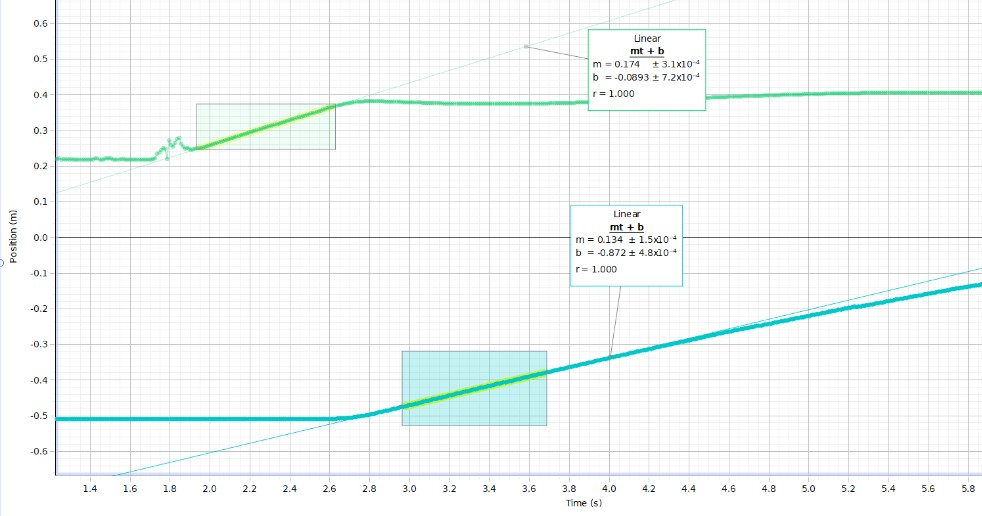
\includegraphics[width=0.8\textwidth]{experiment_1_elastic_collision_velocities.jpg}
    \caption{גרף המתאר את מיקומי העגלות ביחס לזמן}
\end{figure}

נחשב  את התנע הקווי של המערכת לפני ואחרי ההתנגשות, ע"פ נוסחא (2):

\begin{equation*}
    \vec{P_{before}} = 0.49966 \cdot 0.174 + 0.75832 \cdot 0 = 0.087 \, [\frac{kg \cdot m}{s}]
\end{equation*}

\begin{equation*}
    \vec{P_{after}} = 0.49966 \cdot 0 + 0.75832 \cdot 0.134 = 0.1016 \, [\frac{kg \cdot m}{s}]
\end{equation*}

נחשב את השינוי בתנע הקווי של המערכת:

\begin{equation*}
    \Delta \vec{P} = \vec{P_{after}} - \vec{P_{before}} = 0.1016 - 0.087 = 0.0146 \, [\frac{kg \cdot m}{s}]
\end{equation*}

באחוזים נקבל:

\begin{equation*}
    \frac{\Delta \vec{P}}{\vec{P_{before}}} \cdot 100\% = \frac{0.0146}{0.087} \cdot 100\% \approx 16.79\%
\end{equation*}

כלומר נמדדה עליה של בערך 17\% בתנע הכולל.

נחשב את האנרגיה הקינטית לפני ואחרי ההתנגשות:
\begin{center}
    \begin{equation*}
        \begin{aligned}
            \Delta E_k^{before} = \frac{1}{2} m_1 v_1^{i^2} + \frac{1}{2} m_2 v_2^{i^2}                                          \\
            \Delta E_k^{before} = \frac{1}{2} \cdot 0.49966 \cdot 0.174^2 + \frac{1}{2} \cdot 0.75832 \cdot 0^2 = 0.00756 \, [J] \\
            \\
            \Delta E_k^{after} = \frac{1}{2} m_1 v_1^{f^2} + \frac{1}{2} m_2 v_2^{f^2}                                           \\
            \Delta E_k^{after} = \frac{1}{2} \cdot 0.49966 \cdot 0^2 + \frac{1}{2} \cdot 0.75832 \cdot 0.134^2 = 0.00671 \, [J]  \\
            \\
            \Delta E_k = \Delta E_k^{after} - \Delta E_k^{before} = 0.00671 - 0.00756 = -0.00085 \, [J]
        \end{aligned}
    \end{equation*}
\end{center}

כלומר, נאבדה אנרגיה  קינטית בכמות 0.00085 \, [J].

\subsection*{דיון ומסקנות}

בניסוי לא התקיים חוק שימור התנע, והאנרגיה הקינטית לא נשמרה.

כפי שהוצג מקודם, התנע הכולל במערכת עלה ב-17\%.

בגלל שהכוח המגנטי הפועל בין העגלות אינו רגע אלא מתמשך (לפי הגרף בערך 0.1 שניות), אינטרקציה לא מתבצעת "בבת אחת" אלא נמשכת.
הזמן הזה גם רכיב המשקל לאורך המסילה (בהנתן שיפוע קטן במסילה) פועל ברציפות על שתי העגלות.
הכוח הקטן הזה מספיק כדי להוסיף דחף לכיוון התנועה, ועלול להיות הגורם לעלייה בתנע.

נחשב את הזווית הנדרשת על מנת לייצר את המתקף שמאפשר את השינוי בתנע. הזמן האינטרקציה  בין העגלות  הוא בערך 0.1 שניות, וההפרש בין התנע הסופי להתחלתי הוא: $\Delta \vec{P} = 0.0146 \, [\frac{kg \cdot m}{s}]$.

\begin{center}
    \begin{equation*}
        \begin{aligned}
            \Delta p = (m_1 + m_2) \cdot g \cdot \sin(\theta) \cdot \Delta t \\
            \Delta p = (0.49966 + 0.75832) \cdot 9.81 \cdot \sin(\theta) \cdot 0.1 = 0.0146 \, [\frac{kg \cdot m}{s}]
        \end{aligned}
    \end{equation*}
\end{center}

הזווית תנע שמאפשרת את השינוי בתנע היא:

\begin{equation*}
    \sin(\theta) = \frac{\Delta p}{(m_1 + m_2) \cdot g \cdot \Delta t}
    \sin(\theta) = \frac{0.0146}{(0.49966 + 0.75832) \cdot 9.81 \cdot 0.1} \approx 0.7^{\circ}
\end{equation*}

הזווית $0.0677^{\circ}$ קטנה וייתכן שהמסילה הייתה נטויה בזווית זו.

אילו היה נצפה איבוד בתנע, הסיבה העיקרית הייתה יכולה להיות חיכוך עם העגלה ואיבוד אנרגיה קינטית בעת ההתנגשות.

חוסר דיוק  במדידת התנע יכול להווצר כתוצאה מהזמן בו מדדנו את מהירות העגלה.

על מנת לדייק את מדידת התנע, היה נכון למדוד את המהירויות רגע לפני ואחרי ההתנגשות.

כפי שהראנו קודם, גם האנרגיה הקינטית אינה נשמרת. חלק מהאנרגיה הוסבה לצורות אחרות במהלך האינטרקציה, חיכוך בגלגלים ובמסילה הפך חלק מהאנרגיה לחום.

איזון המסילה נעשה בעזרת פלס, והנחת עגלה במקומות שונים במסילה, ווידוא שהיא לא זזה כתוצאה משיפוע.

שגיאת המדידה של  המהירות לפני ההתנגשות ניתנה מהגרף (ע"י התוכנה)  וערכה $3.1 \cdot 10^{-4} \, [\frac{m}{s}]$. ולכן השגיאה בחישוב התנע ההתחלתי היא:
\begin{equation*}
    \sigma_p = m_{\textbf{כחול}} \cdot \sigma_{\textbf{כחול}} + m_{\textbf{אדום}} \cdot \sigma_{\textbf{אדום}} = 0.49966 \cdot 3.1 \cdot 10^{-4} + 0.75832 \cdot 0 = 1.55 \cdot 10^{-4} \, [\frac{kg \cdot m}{s}]
\end{equation*}
שגיאת המהירות אחרי ההתנגשות ניתנה גם היא מהגרף וערכה $1.5 \cdot 10^{-4} \, [\frac{m}{s}]$. ולכן השגיאה בחישוב התנע הסופי היא:
\begin{equation*}
    \sigma_p = m_{\textbf{כחול}} \cdot \sigma_{\textbf{כחול}} + m_{\textbf{אדום}} \cdot \sigma_{\textbf{אדום}} = 0.49966 \cdot 0 + 0.75832 \cdot  1.5 \cdot 10^{-4} = 7.5 \cdot 10^{-5} \, [\frac{kg \cdot m}{s}]
\end{equation*}

\section*{ניסוי 2 - התנגשות פלסטית בין עגלות}
\subsection*{מטרת הניסוי}
בחינת חוק שימור התנע ושימור האנרגיה הקינטית על ידי התנגשות חד ממדית בין שתי עגלות.
\subsection*{רקע תיאורטי}
נעזר באותן נוסחאות תנע שהוצגו בניסוי 1

חשוב לציין שההתנגשות בניסוי זה היא פלסטית, כלומר לאחר ההתנגשות הגופים נעים ביחס ולא מצופה שתשמר האנרגיה הקינטית.

\subsection*{מערכת המדידה ומהלך הניסוי}
בניסוי זה חזרנו על נעשה בניסוי 1, אז  הפעם מיקמנו את העגלות כך שהן יידבקו לאחר ההתנגשות.

\subsection*{תוצאות וניתוח}

תוצאות הניסוי מתוארות בטבלה הבאה:

\begin{table}[H]
    \centering
    \renewcommand{\arraystretch}{1.5} % Increase row height
    \begin{tabular}{|c|c|}
        \hline
        מסת עגלה כחולה - m1 (kg)                            & 0.49966 \\
        \hline
        מסת עגלה אדומה - m2 (kg)                            & 0.75832 \\
        \hline
        מהירות התחלתית עגלה כחולה - $v_{1}^i [\frac{m}{s}]$ & 0.365   \\
        \hline
        מהירות התחלתית עגלה אדומה - $v_{2}^i [\frac{m}{s}]$ & 0       \\
        \hline
        מהירות סופית עגלה כחולה - $v_{1}^f [\frac{m}{s}]$   & 0.146   \\
        \hline
        מהירות סופית עגלה אדומה - $v_{2}^f [\frac{m}{s}]$   & 0.14    \\
        \hline
    \end{tabular}
    \caption{תאוצת העגלה בזוויות שונות}
\end{table}

מיקום העגלות לפני ואחרי התנגשות מתואר בגרף הבא. הגרף העליון מתאר את העגלה הכחולה והגרף התחתון את העגלה האדומה:

\begin{center}
    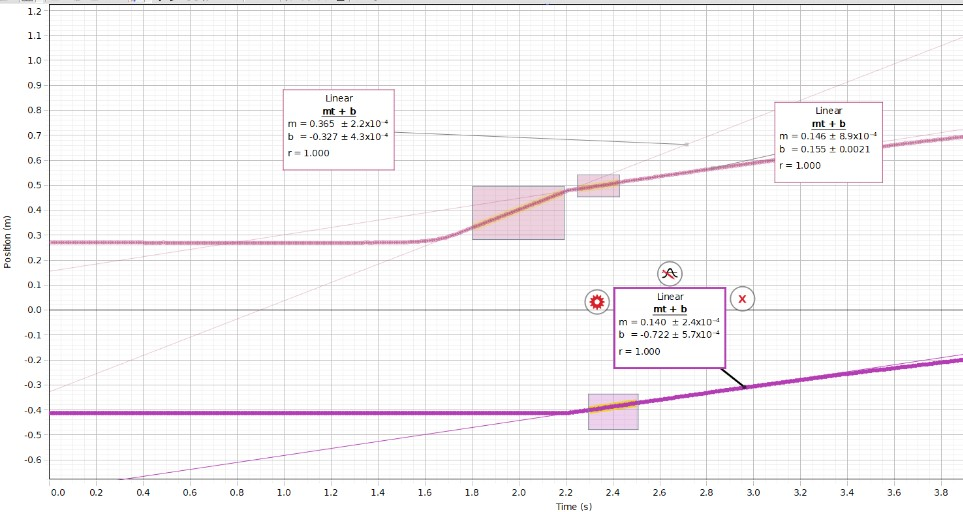
\includegraphics[width=0.8\textwidth]{experiment_2_plastic_collision.jpg}
\end{center}

נחשב את התנע הקווי לפני ההתנגשות. השגיאה במהירות נלקחה מההתאמה הליניארית שנעשתה ע"י התוכנה.

\begin{equation*}
    \vec{P_{before}} = 0.49966 \cdot 0.365 + 0.75832 \cdot 0 = 0.1813 \, [\frac{kg \cdot m}{s}]
\end{equation*}
\begin{equation*}
    \sigma_p = \textbf{שגיאה} = m_{\textbf{כחול}} \cdot 2.2 \cdot 10^{-4} = 1.1 \cdot 10^{-4} \, [\frac{kg \cdot m}{s}]
\end{equation*}

נחשב את התנע הקווי אחרי ההתנגשות. השגיאה במהירות נלקחה מההתאמה הליניארית שנעשתה ע"י התוכנה.

\begin{equation*}
    \vec{P_{after}} = 0.49966 \cdot 0.146 + 0.75832 \cdot 0.14 = 0.1791 \, [\frac{kg \cdot m}{s}]
\end{equation*}
\begin{center}
    \begin{equation*}
        \begin{aligned}
            \sigma_p = \textbf{שגיאה} = \sqrt{(m_{\textbf{כחול}} \cdot \sigma_{\textbf{כחול}})^2 + (m_{\textbf{אדום}} \cdot \sigma_{\textbf{אדום}})^2} \\
            \sigma_p = \sqrt{(0.49966 \cdot 8.9 \cdot 10^{-4})^2 + (0.75832 \cdot 2.4 \cdot 10^{-4})^2} =  4.8 \cdot 10^{-4} \, [\frac{kg \cdot m}{s}]
        \end{aligned}
    \end{equation*}
\end{center}

התנע הקווי אינו נשמר.

נחשב  את  אובדן האנרגיה  הקינטית:
\begin{center}
    \begin{equation*}
        \begin{aligned}
            E_k^{before} = \frac{1}{2} m_1 v_1^{i^2} + \frac{1}{2} m_2 v_2^{i^2} = \frac{1}{2} \cdot 0.49966 \cdot 0.365^2 + \frac{1}{2} \cdot 0.75832 \cdot 0^2 = 0.0333 \, [J]   \\
            E_k^{after} = \frac{1}{2} m_1 v_1^{i^2} + \frac{1}{2} m_2 v_2^{i^2} = \frac{1}{2} \cdot 0.49966 \cdot 0.146^2 + \frac{1}{2} \cdot 0.75832 \cdot 0.14^2 = 0.0127 \, [J] \\
            \Delta E_k = 0.333 - 0.0127 = 0.0205 \, [J]                                                                                                                            \\
        \end{aligned}
    \end{equation*}
\end{center}

בניסוי הראשון אבדה 0.00085 \, [J] מהאנרגיה הקינטית, ואילו בניסוי הזה אבדה 0.0205 \, [J], כלומר פי 24 מהניסוי הראשון.

\subsection*{דיון ומסקנות}

בניסוי זה לא התקיים חוק שימור התנע, והאנרגיה הקינטית לא נשמרה.

אחת התופעות שרואים בגרף היא שאפילו שהעגלות נעות ביחד  לאחר ההתנגשות המהירות שלהן שונה במעט.

שגיאת המדידה לא מסבירה את ההפרש בין המהירויות, סיבה יותר  הגיונית היא שחלון המדידה של המהירויות נמדד בזמנים מעט שונים.
כיוון והעגלות  מאטות כתוצאה מחיכוך, אז אם חלונות המדידה בזמנים שונים המהירויות עלולות להיות שונות.

לפי התיאוריה התנע הכולל אמור להשמר, אך בניסוי הוא לא נשמר. ההפרש בתנע שווה ל $2.2\cdot 10^{-4} \, [\frac{kg \cdot m}{s}]$.

ניתן לייחס את  חוסר שימור התנע  והאנרגיה  הקינטית לחיכוך. האנרגיה  הקינטית ש"אבדה" כנראה הומרה לחום.

\section*{ניסוי 3 - מתקף ותנע}
\subsection*{מטרת הניסוי}
מדידת מתקף ותנע של התנגשות בין עגלה לבין קפיצים שונים, ופלסטלינה.

\subsection*{רקע תיאורטי}
הגדרת מתקף היא:
\begin{equation}
    \vec{J} = \int_{t_final}^{t_initial} \vec{F} \, dt
\end{equation}
כלומר, כאשר פועל כוח $\vec{F}$ לאורך זמן  $t$, אז המתקף הוא  האינטגרל של הכוח ביחס לזמן (השטח שמתחת לגרף הכוח כתלות בזמן).

משפט מתקף-תנע קובע  כי  השינוי בתנע  הקווי של גוף כלשהו שווה למתקף הפועל על אותו גוף:
\begin{equation}
    \vec{J} = \Delta \vec{P} = \vec{P_{final}} - \vec{P_{initial}}
\end{equation}

\subsection*{מערכת המדידה ומהלך הניסוי}
בקצה אחד של מסילה הרכבנו  חיישן תנועה, ובקצה  השני  הרכבנו חיישן כוח.

הגבהנו צד אחד של המסילה כדי ליצור שיפוע קטן.

לאחר מכן שחררנו עגלה ממרחק 40 ס"מ מחיישן התנועה מספר פעמים, כך שכל פעם הייתה התנגשות אחרת. בכל פעם מדדנו  את מסת העגלה, המתקף, והמהירות  לפני  ואחרי ההתנגשות.

\subsection*{תוצאות וניתוח}

ראשית נציג את תוצאות המדידות:

\begin{table}[H]
    \centering
    \begin{tabular}{|c|p{2cm}|p{2cm}|p{2cm}|p{2cm}|}
        \hline
                                                      & קפיץ 1 עגלה ללא משקולת & קפיץ 1 עגלה עם משקולת  & קפיץ 2 עגלה ללא משקולת & פלסטלינה              \\
        \hline
        מסת העגלה m [Kg]                              & 0.2508                 & 0.4966                 & 0.2508                 & 0.2508                \\
        \hline
        מתקף J [N·s]                                  & 0.068                  & 0.115                  & 0.055                   & 0.032                  \\
        \hline
        מהירות לפני $v_i [\frac{m}{s}]$               & 0.13                   & 0.12                   & 0.11                   & 0.12                  \\
        \hline
        מהירות אחרי $v_f [\frac{m}{s}]$               & 0.12-                  & 0.1-                   & 0.09-                  & 0                     \\
        \hline
        תנע לפני $P_i [\frac{kg \cdot m}{s}]$         & 0.0326                 & 0.0599                 & 0.0276                 & 0.0301                \\
        \hline
        תנע אחרי $P_f [\frac{kg \cdot m}{s}]$         & 0.0301-                & 0.0499-                & 0.0226-                & 0                     \\
        \hline
        שינוי בתנע  $\Delta P [\frac{kg \cdot m}{s}]$ & 0.0627-                & 0.1098-                & 0.0502-                & 0.0301-               \\
        \hline
        אנרגיה קינטית לפני $E_k^i [J]$                & $2.12 \cdot 10^{-3}$   & $3.59 \cdot 10^{-3}$   & $1.52 \cdot 10^{-3}$   & $1.8 \cdot 10^{-3}$   \\
        \hline
        אנרגיה קינטית אחרי $E_k^f [J]$                & $1.8 \cdot 10^{-3}$    & $2.5 \cdot 10^{-3}$    & $1.01 \cdot 10^{-3}$   & 0                     \\
        \hline
        שינוי באנרגיה קינטית $\Delta E_k [J]$         & $-3.2 \cdotp 10^{-4}$  & $-1.09 \cdotp 10^{-3}$ & $-5.1 \cdotp 10^{-4}$  & $-1.8 \cdotp 10^{-3}$ \\
        \hline
    \end{tabular}
\end{table}

מצ"ב הגרפים המתארים את המהירות והכוח כתלות בזמן בכל אחד מהניסויים, מהם נלקחו נתוני המהירות והמתקף:

\begin{figure}[H]
    \centering
    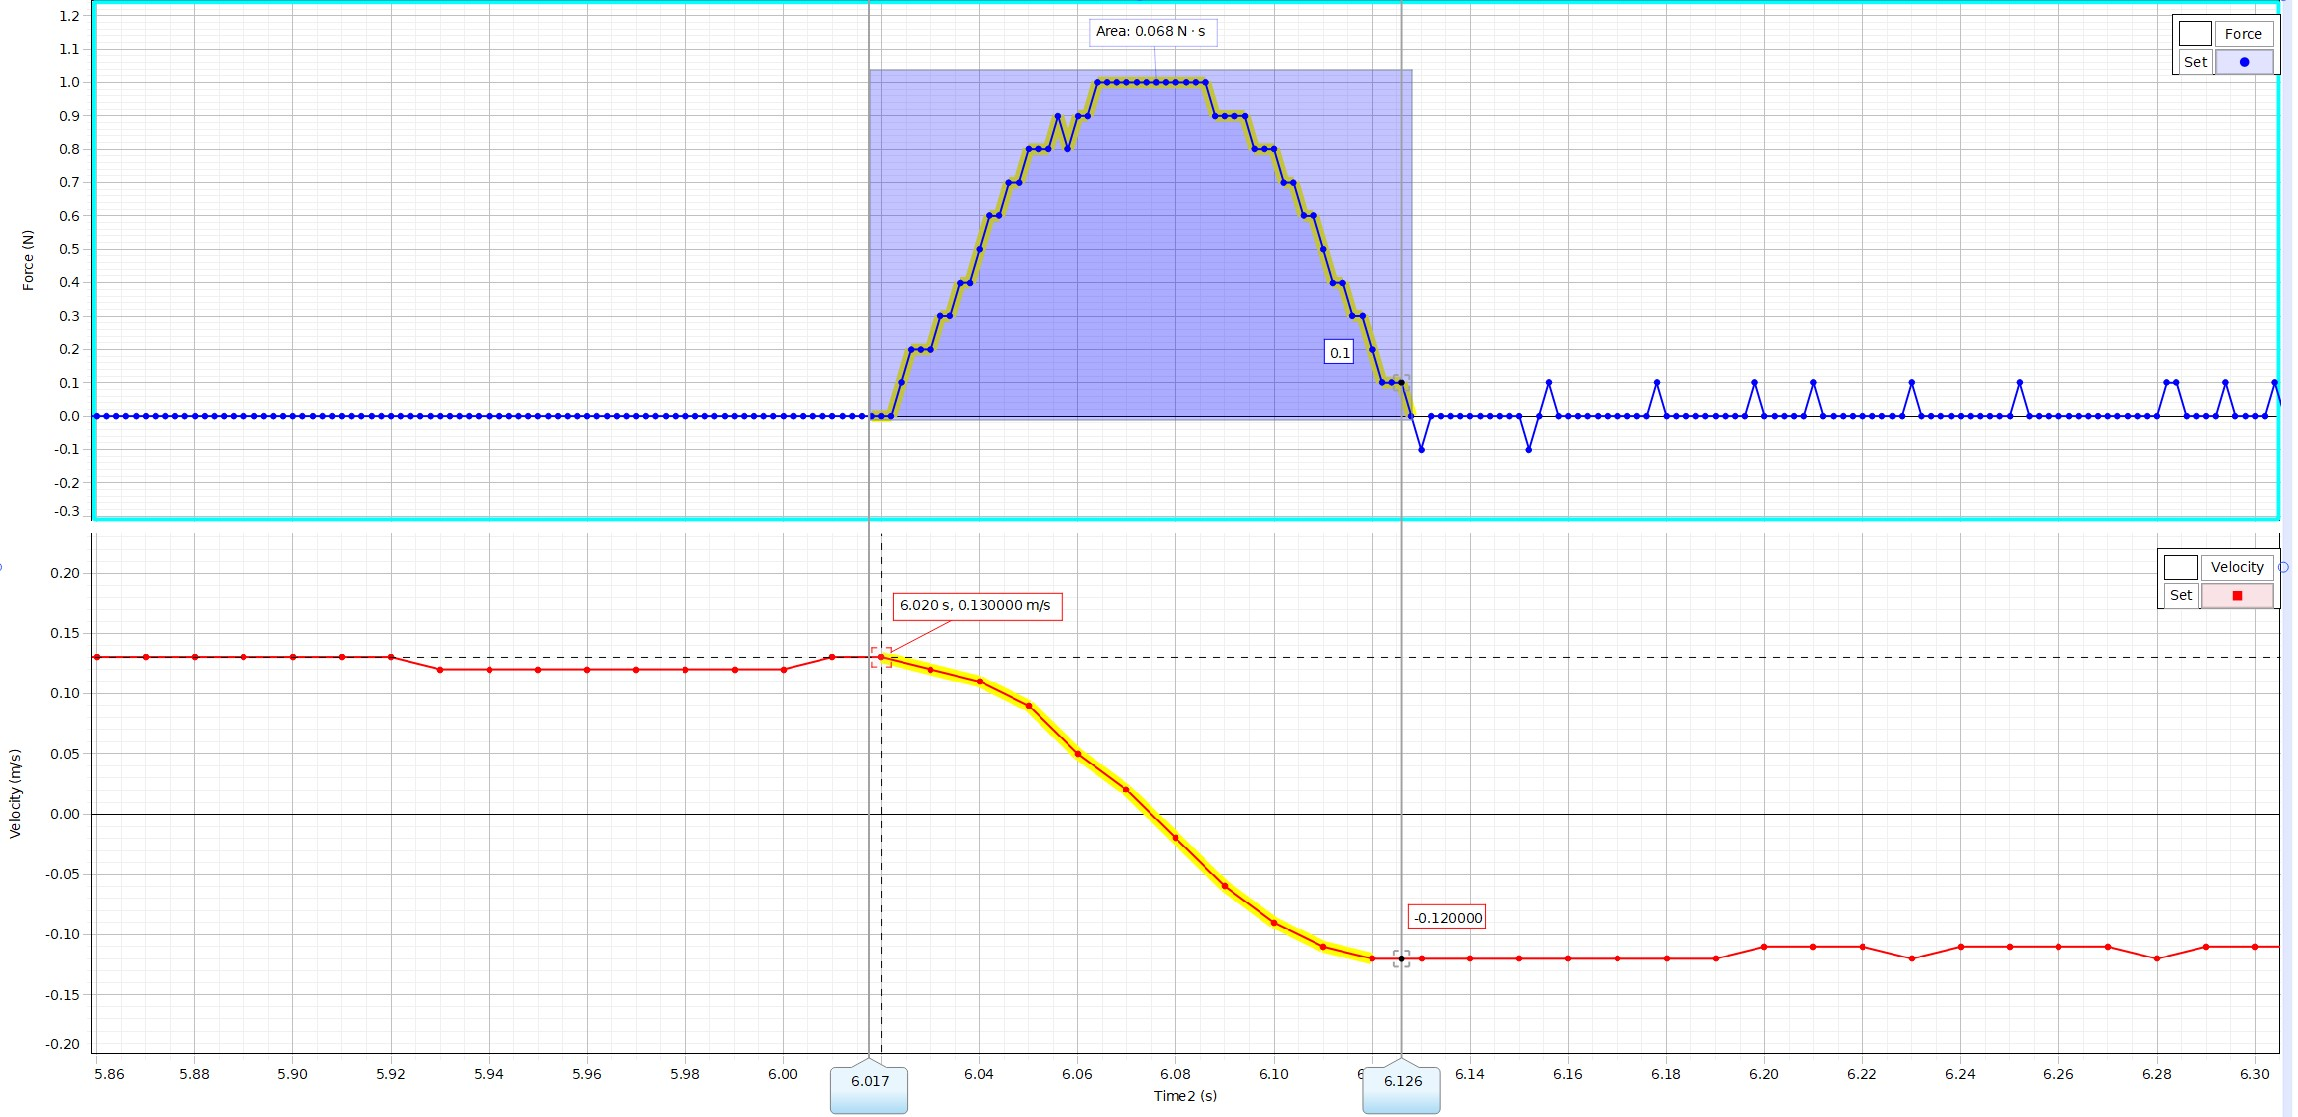
\includegraphics[width=0.8\textwidth]{experiment_3_spring_1_without_weight.jpg}
    \caption{קפיץ 1  עגלה ללא משקולת}
\end{figure}

\begin{figure}[H]
    \centering
    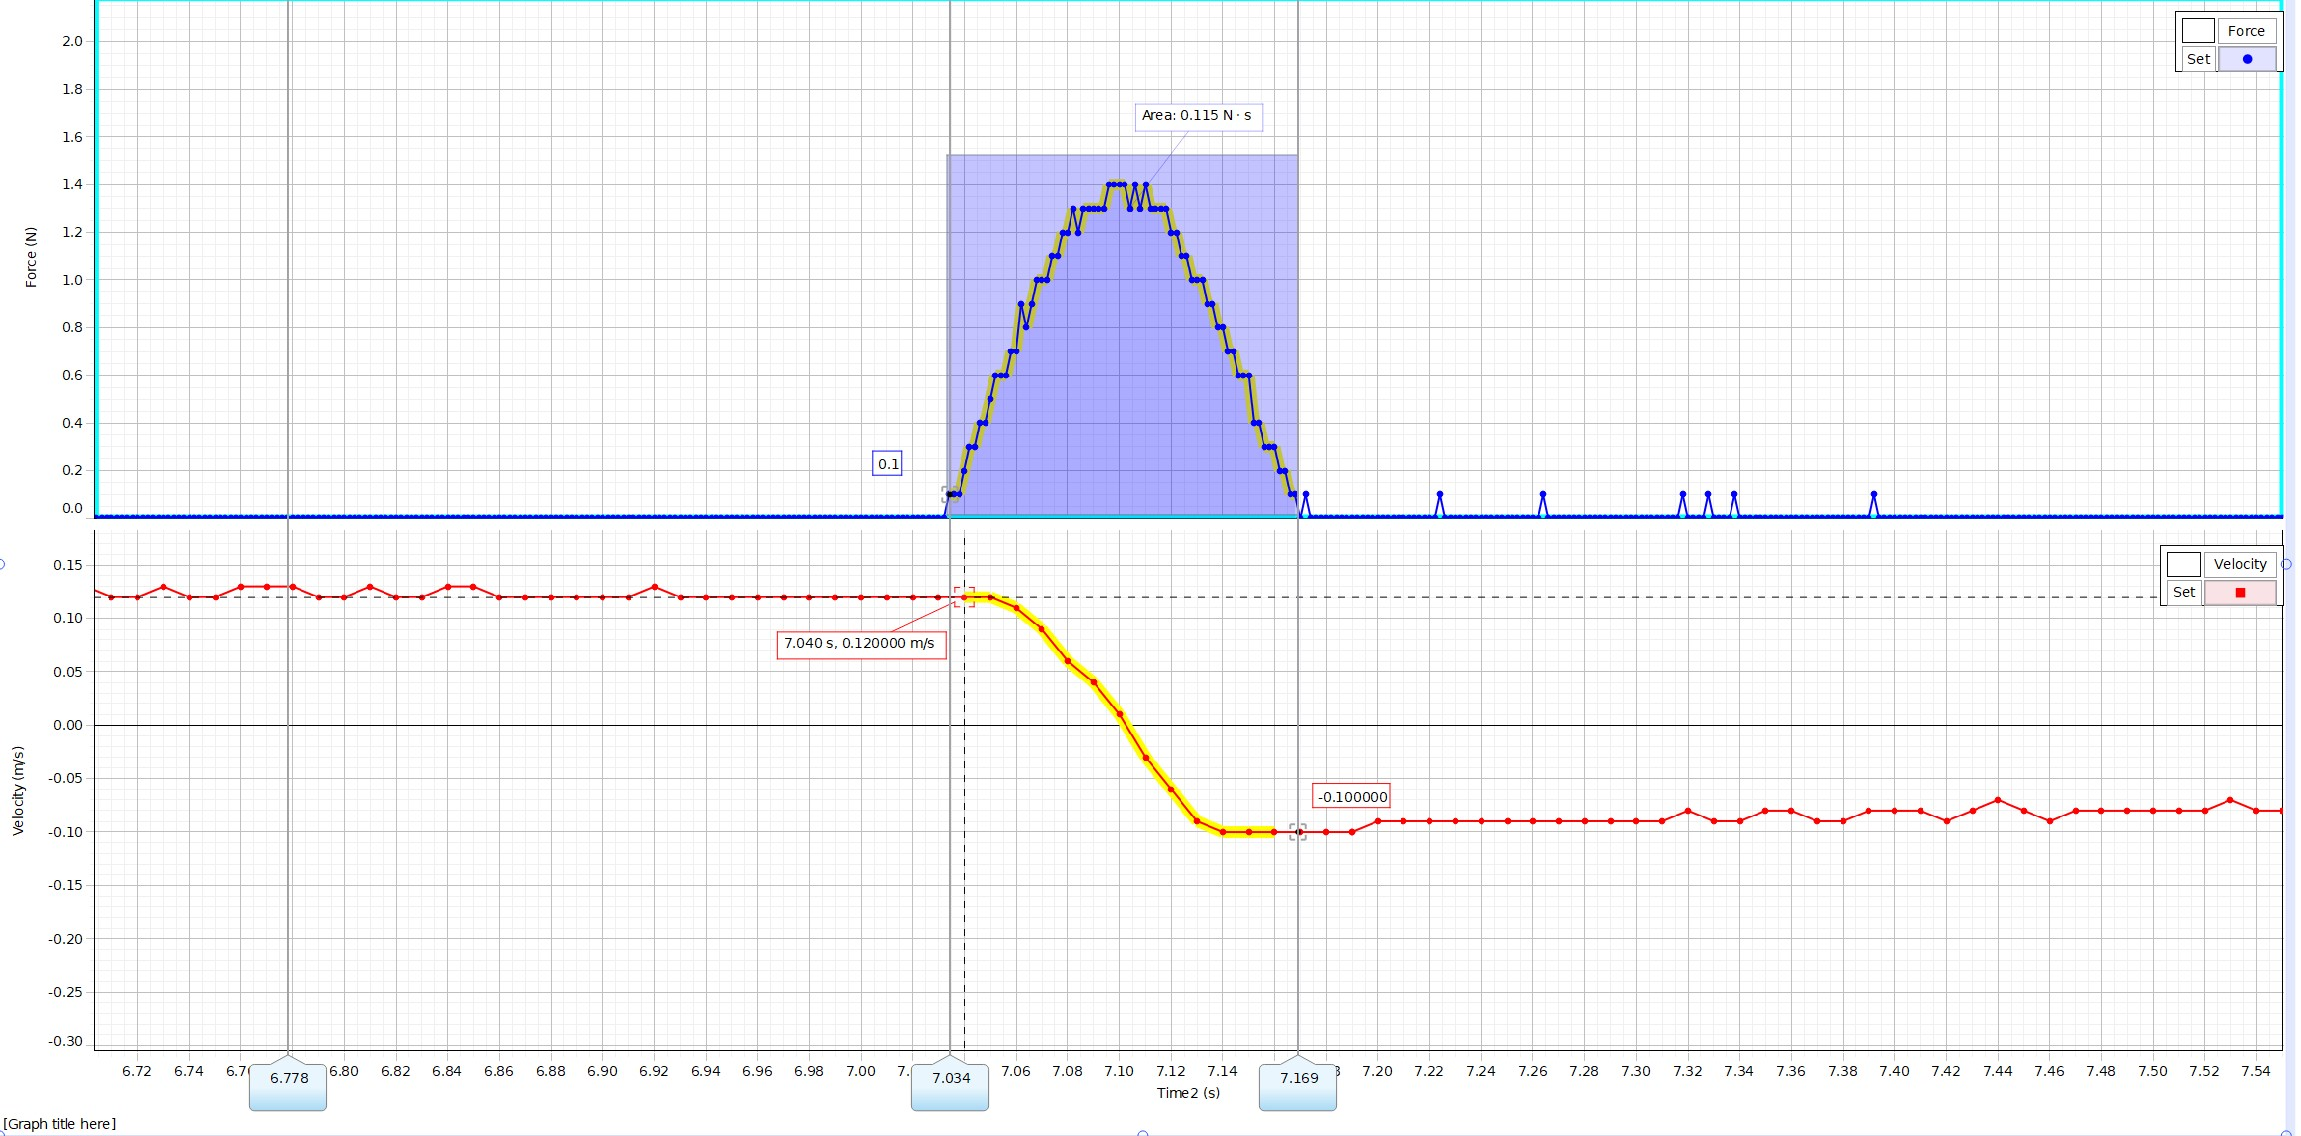
\includegraphics[width=0.8\textwidth]{experiment_3_spring_1_with_weight.jpg}
    \caption{קפיץ 1  עגלה עם משקולת}
\end{figure}

\begin{figure}[H]
    \centering
    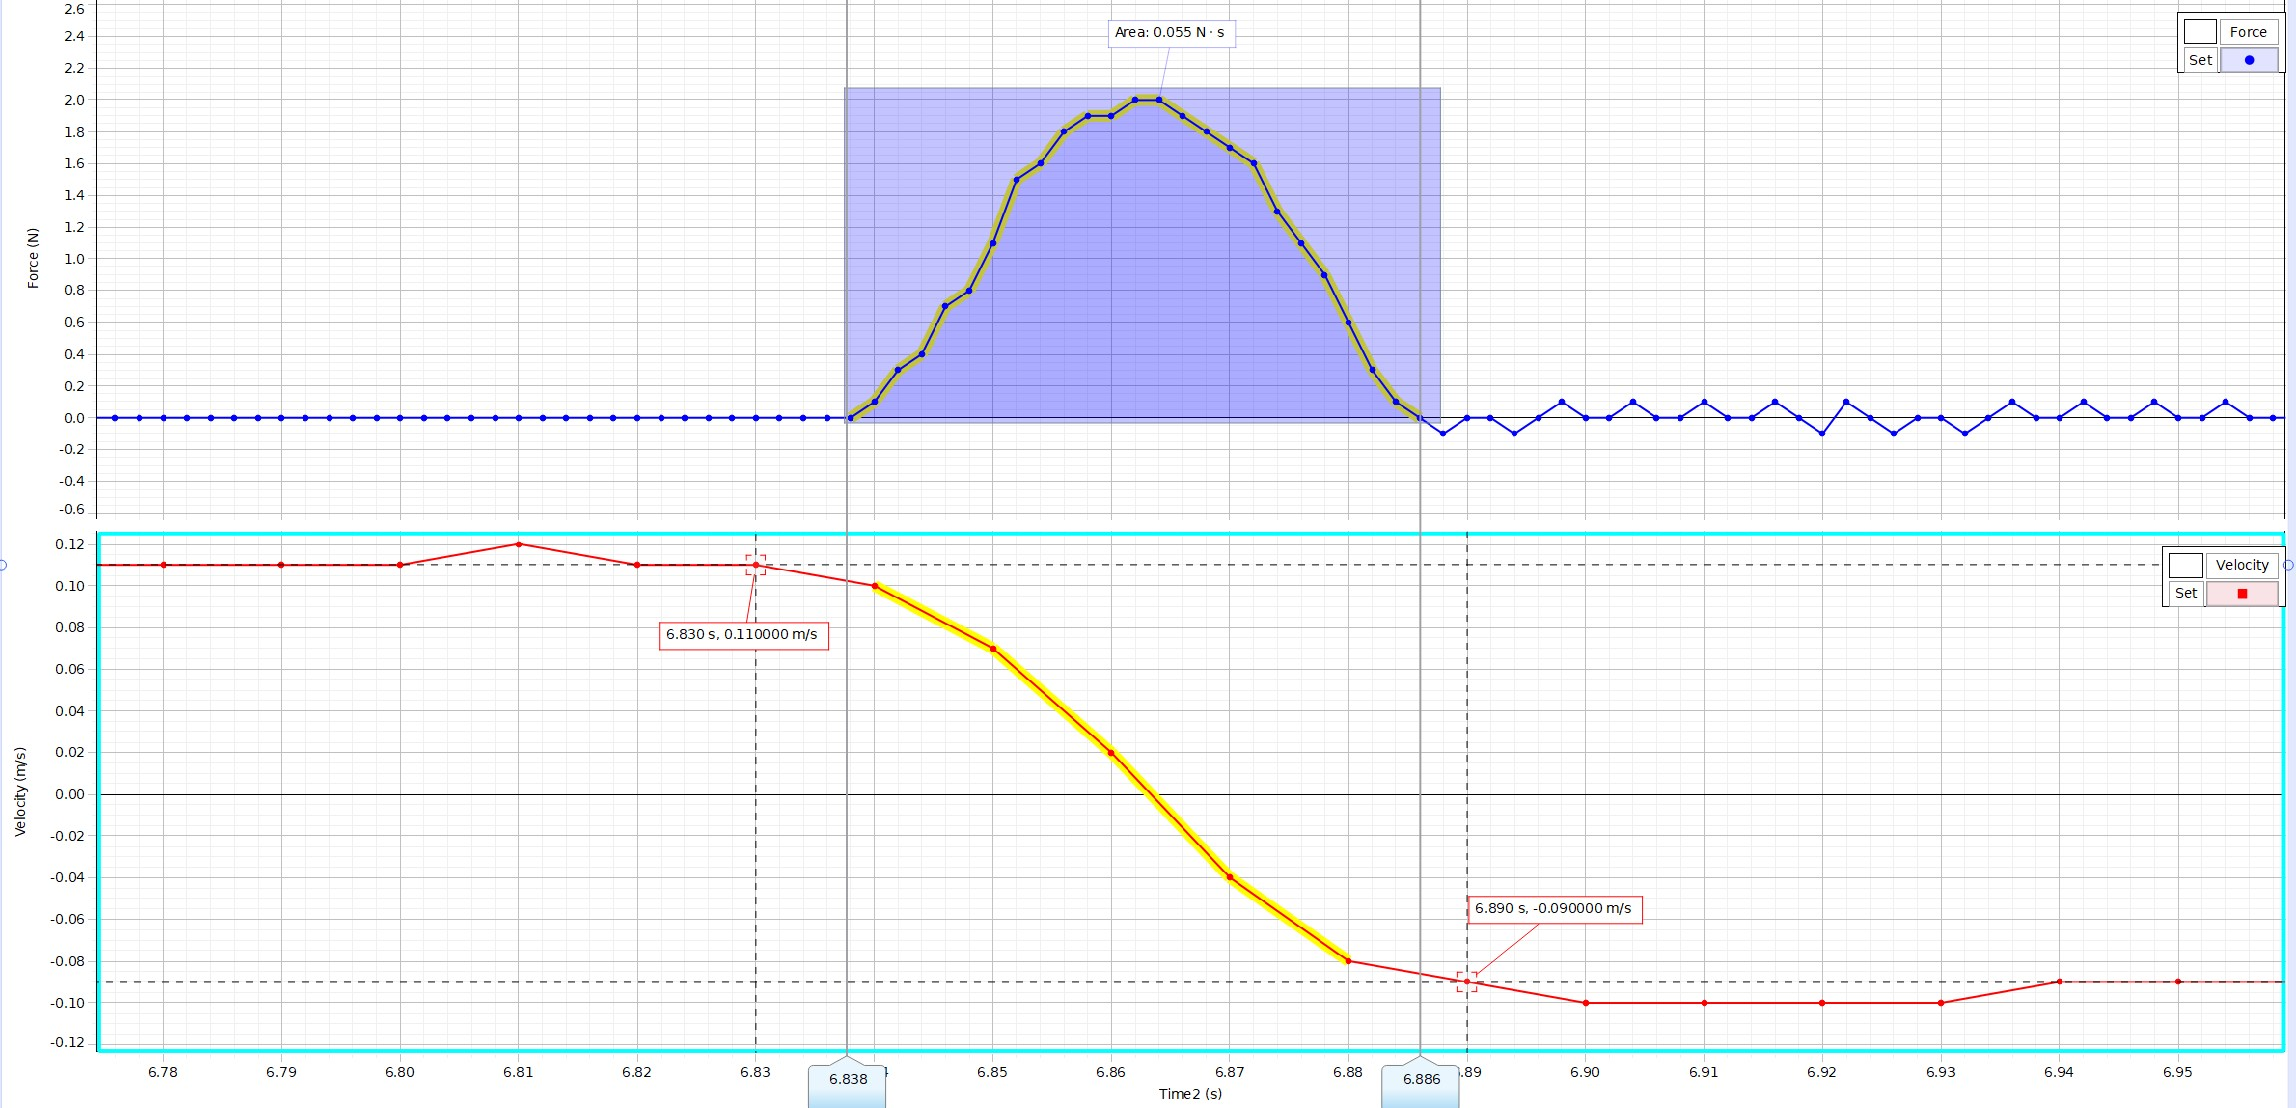
\includegraphics[width=0.8\textwidth]{experiment_3_spring_2_without_weight.jpg}
    \caption{קפיץ 2 עגלה ללא משקולת}
\end{figure}

\begin{figure}[H]
    \centering
    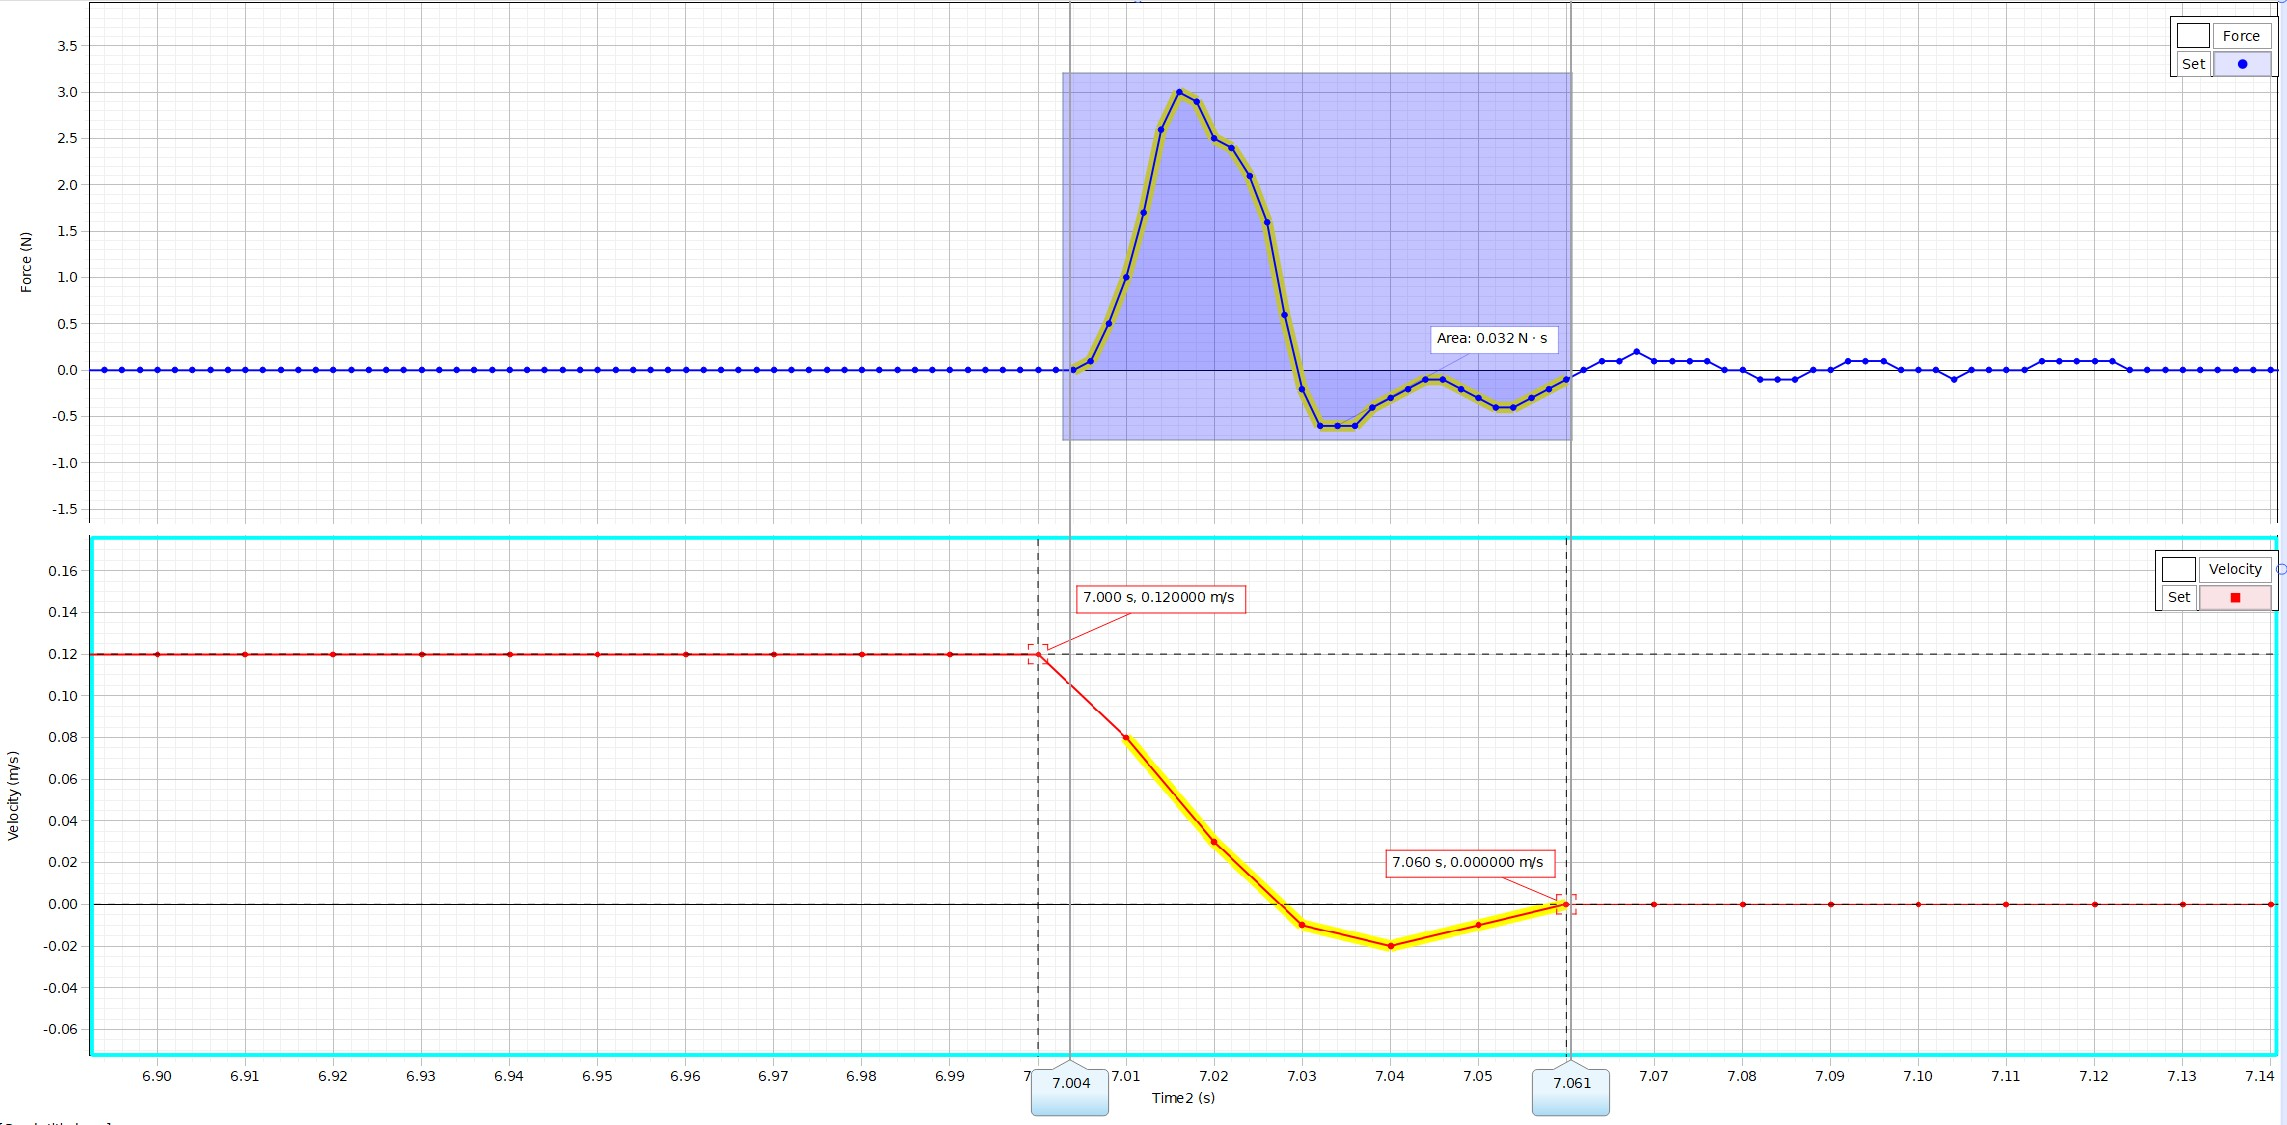
\includegraphics[width=0.8\textwidth]{experiment_3_plastelina_without_weight.jpg}
    \renewcommand{\arraystretch}{1.5} % Increase row height
    \caption{פלסטלינה עגלה ללא משקולת}
\end{figure}


\subsection*{דיון ומסקנות}

את ההבדלים באנרגיה הקינטית בכל ניסוי ניתן לראות בטבלה, וכן את השינוי בתנע (מתקף).

את המתקף ניתן גם לקבל מהשטח מתחת לגרף הכוח כתלות בזמן.

נחשב את השגיאה היחסית בכל אחד מהניסויים:
\begin{center}
    \begin{equation*}
        \begin{aligned}
            \sigma_{\textbf{קפיץ 1 ללא משקל}} = \frac{|0.068 - 0.0627|}{\frac{0.068 + 0.0627}{2}} \cdot 100\% = 8.11\% \\
            \sigma_{\textbf{קפיץ 1 עם משקל}} = \frac{|0.115 - 0.1098|}{\frac{0.115 + 0.1098}{2}} \cdot 100\% = 4.62\% \\
            \sigma_{\textbf{קפיץ 2 ללא משקל}} = \frac{|0.055 - 0.0502|}{\frac{0.055 + 0.0502}{2}} \cdot 100\% = 9.12\% \\
            \sigma_{\textbf{פלסטלינה ללא משקל}} = \frac{|0.032 - 0.0301|}{\frac{0.032 + 0.0301}{2}} \cdot 100\% = 6.12\% \\
        \end{aligned}
    \end{equation*}
\end{center}

ניתן לראות שבשני הקפיצים צורת גרף הכוח היא פרבולה. ככל שהקפיץ מתכווץ הכוח שהוא מפעיל על העגלה גדל, כצפוי.

כאשר העגלה ללא המשקולת התנגשה בקפיץ הראשון, משך ההתנגשות   היה 0.11 שניות, וכאשר התנגשה בקפיץ השני משך ההתנגשות  היה  0.048 שניות (ערכים אלו נלקחו מהגרפים).
כלומר, הקפיץ השני אלסטי יותר (מחזיר את  האנרגיה בזמן קצר יותר), והקפיץ הראשון פחות אלסטי.

ניתן לראות שבהתנגשות עגלה במשקל שונה עם אותו הקפיץ גודל המתקף גדל משמעותית (כאשר המשקל גדול יותר), ניתן לנמק זאת בכך שהשינוי במהירות היה משמעותי יותר וכן השינוי בתנע, כאשר המסה גדולה יותר.

עם זאת, ניתן לראות שמשך זמן ההתנגשות דומה, לכן המסה משפיעה על גודל המתקף אבל לא על זמן ההתנגשות, שתלוי בעיקר בקבוע הקפיץ.

בפלסטלינה לעומת זאת ניתן לראות שמלוא האנרגיה הקינטית אבדה. וכן המתקף קטן יותר כיוון והעגלה לא נעה לכיוון השני לאחר ההתנגשות (בניגוד לקפיצים).

\end{document}